\documentclass[a4paper,10pt]{article} 
\usepackage[utf8]{inputenc}
\usepackage[a4paper]{geometry}
\usepackage[magyar]{babel}
\usepackage{amsmath}
\usepackage{amssymb}
\usepackage{pgf,tikz}
\usetikzlibrary{arrows}
\usepackage{caption}
\frenchspacing 
\pagestyle{empty}
\newcommand{\ki}[2]{\hfill {\it #1 (#2)}\medskip}
\newcommand{\vonal}{\hbox to \hsize{\hskip2truecm\hrulefill\hskip2truecm}}
\newcommand{\degre}{\ensuremath{^\circ}}
\newcommand{\tg}{\mathop{\mathrm{tg}}\nolimits}
\newcommand{\ctg}{\mathop{\mathrm{ctg}}\nolimits}
\newcommand{\arc}{\mathop{\mathrm{arc}}\nolimits}
\begin{document}
\begin{center} \Large {\em XX. Nemzetközi Magyar Matematika Verseny} \end{center}
\begin{center} \large{\em Bonyhád, 2011. március 11--15.} \end{center}
\smallskip
\begin{center} \large{\bf 9. osztály} \end{center}
\bigskip 

{\bf 1. feladat: } ,,Fanyűvő és én együtt 20 nap alatt vágnánk ki a Nagy Kerek Erdőt'' -- mondja Törzsök Jankó. ,,Bár ha Erdődöntögetővel dolgoznék, akkor ezt a munkát öt nappal előbb befejeznénk.'' ,,Nekem jobb ötletem van'' -- mondja Erdődöntögető. ,,Ha én dolgoznék együtt Fanyűvővel, akkor mi ketten egy ötödével kevesebb idő alatt végeznénk a munkával, mint ha Törzsök Jankóval dolgoznék.'' Mennyi idő alatt vágnák ki a Nagy Kerek Erdőt külön-külön ezek az erős emberek, és mennyi idő alatt végeznének a munkával, ha mindhárman együtt dolgoznának?

\ki{Peics Hajnalka}{Szabadka}\medskip


{\bf Megoldás: } Jelölje $x$, $y$ illetve $z$, ugyanebben a sorrendben azon napoknak a számát, amelyek alatt Fanyűvő, Törzsök Jankó illetve Erdődöngető kivágná a Nagy Kerek Erdőt. Ha az elvégzendő munkát 1-gyel jelöljük, akkor Fanyűvő, Törzsök Jankó illetve Erdődöngető a munka $\frac1x$, $\frac1y$ illetve $\frac1z$ részét végezné el egy nap alatt. A feladat feltételei alapján felírhatjuk a következő e\-gyen\-let\-rend\-szert:
\begin{equation*}
\left.
\begin{aligned}
\frac1x+\frac1y&=\frac{1}{20} \\
\frac1y+\frac1z&=\frac{1}{15} \\
\frac1x+\frac1z&=\frac{1}{12} \\
\end{aligned}
\right\}
\end{equation*}

A fenti háromismeretlenes egyenletrendszert kell megoldani.

Összeadva a három egyenletet, némi rendezés után azt kapjuk, hogy
\[\frac1x+\frac1y+\frac1z=\frac{1}{10}.\]

Ez azt jelenti, hogy mindhárman együtt dolgozva egy nap alatt a munka $\frac{1}{10}$ részét végeznék el, a teljes munkát pedig 10 nap alatt.

Ebből adódik, hogy
\[\frac1x=\frac{1}{10}-\left(\frac1y+\frac1z\right)=\frac{1}{10}-\frac{1}{15}=\frac{1}{30},\]
vagyis $x=30$.

Hasonló módon kapjuk, hogy $y=60$, $z=20$.

Tehát a Nagy Kerek Erdőt Fanyűvő 30 nap alatt, Törzsök Jankó 60 nap alatt, Erdődöngető pedig 20 nap alatt vágná ki.
\medskip


\vonal
{\bf 2. feladat: } Bizonyítsuk be, hogy minden $n\in\mathbb{N}^+$ számra a $(2n+1)^2+(2n+2)^2+(2n+3)^2$ kifejezés felírható 4 különböző pozitív egész szám négyzetösszegeként.

\ki{Bencze Mihály}{Brassó}\medskip

{\bf Megoldás: } Jelöljük (az egyszerűség kedvéért) a középső számot $2n+2=2a$-val ($n=a-1$). Így a következőt kellene belátni:
\[(2a-1)^2+(2a)^2+(2a+1)^2\]
felbontható 4 különböző négyzetszám összegére.

Elvégezve a kijelölt műveleteket és csoportosítva:
\begin{multline*}
(2a-1)^2+(2a)^2+(2a+1)^2=4a^2-4a+1+4a^2+4a^2+4a+1=\\
=12a^2+2=a^2-2a+1+a^2+a^2+2a+1+9a^2=(a-1)^2+a^2+(a+1)^2+(3a)^2
\end{multline*}

Mivel $a-1<a<a+1$, ezért ezek különbözők, ha
\[a-1\ne3a \textrm{ és } a\ne3a \textrm{ és } a+1\ne3a\]

Ezek teljesülnek, hiszen $a$ pozitív egész szám. Visszatérve $n$-re:
\[(a-1)^2+a^2+(a+1)^2+(3a)^2=n^2+(n+1)^2+(n+2)^2+(3n+3)^2\]
a keresett felbontás.
\medskip


\vonal
{\bf 3. feladat: } 
Az $ABC$ egyenlő szárú háromszögben $A\sphericalangle=100^\circ$. Vegyük fel az $AB$ szár $B$-n túli meghosszabbításán a $D$ pontot úgy, hogy $AD=BC$ legyen. Mekkorák a $BCD$ háromszög szögei?

\ki{Katz Sándor}{Bonyhád}\medskip

{\bf Megoldás: } $ABC\sphericalangle=40^\circ \Rightarrow DBC\sphericalangle=140^\circ$ (kiegészítő szögek).

$AD=BC$, ezért vegyük fel az eredetivel egybevágó $ADE$ háromszöget!
\begin{figure}[hbp!]
\begin{center}
{
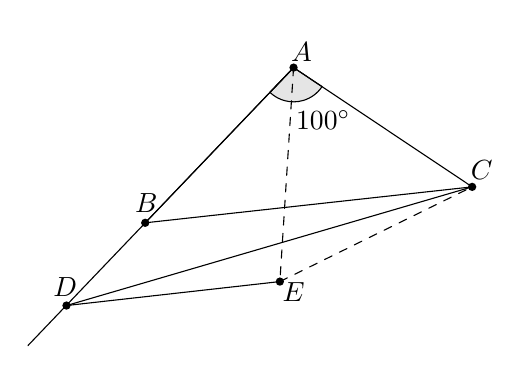
\begin{tikzpicture}[line cap=round,line join=round,>=triangle 45,x=0.7246376811594202cm,y=0.7246376811594202cm]
\clip(-3.32,-0.3) rectangle (4.96,5.38);
\draw [shift={(1.34,4.68)},fill=black,fill opacity=0.1] (0,0) -- (-133.71:0.6) arc (-133.71:-33.71:0.6) -- cycle;
\draw (1.34,4.68)-- (-1.26,1.96);
\draw (-1.26,1.96)-- (4.47,2.59);
\draw (4.47,2.59)-- (1.34,4.68);
\draw [domain=-3.3200000000000003:1.34] plot(\x,{(-8.52-2.72*\x)/-2.6});
\draw (-2.64,0.51)-- (4.47,2.59);
\draw [dash pattern=on 3pt off 3pt] (1.34,4.68)-- (1.1,0.93);
\draw [dash pattern=on 3pt off 3pt] (1.1,0.93)-- (4.47,2.59);
\draw (1.1,0.93)-- (-2.64,0.51);
\fill [color=black] (1.34,4.68) circle (1.5pt);
\draw[color=black] (1.48,4.96) node {$A$};
\fill [color=black] (-1.26,1.96) circle (1.5pt);
\draw[color=black] (-1.24,2.3) node {$B$};
\fill [color=black] (4.47,2.59) circle (1.5pt);
\draw[color=black] (4.64,2.88) node {$C$};
\fill [color=black] (-2.64,0.51) circle (1.5pt);
\draw[color=black] (-2.66,0.84) node {$D$};
\fill [color=black] (1.1,0.93) circle (1.5pt);
\draw[color=black] (1.34,0.74) node {$E$};
\draw[color=black] (1.86,3.76) node {$100\textrm{\degre}$};
\end{tikzpicture}
}
\end{center}
\caption*{A 3. feladathoz.}
\end{figure}
$DAE\sphericalangle=40^\circ$ (az egybevágóság miatt) $\Rightarrow EAC\sphericalangle=100^\circ-40^\circ=60^\circ$.

$AE=AC$ (az egybevágóság miatt) $\Rightarrow$ az $AEC$ háromszög szabályos (egyenlő szárú és egyik szöge $60^\circ$), $AEC\sphericalangle=ACE\sphericalangle=60^\circ$.

$DEC\sphericalangle=100^\circ+60^\circ=160^\circ$.

$DE=ED \Rightarrow EDC\sphericalangle=ECD\sphericalangle=10^\circ$.

$DCB\sphericalangle=ACE\sphericalangle-ECD\sphericalangle-ACB\sphericalangle=60^\circ-10^\circ-40^\circ=10^\circ$.

$BDC\sphericalangle=180^\circ-DBC\sphericalangle-BCD\sphericalangle=180^\circ-140^\circ-10^\circ=30^\circ$.

Tehát a háromszög szögei $140^\circ$, $30^\circ$ és $10^\circ$.
\medskip


\vonal
{\bf 4. feladat: } 
Az $ABC$ háromszög $AB$, $BC$, $CA$ oldalait meghosszabbítjuk a $B$, $C$ és $A$ pontokon túl a $BB_1$, $CC_1$, $AA_1$ szakaszokkal úgy, hogy $BB_1=AC$, $CC_1=AB$, $AA_1=BC$ legyen. Jelölje továbbá az $ABC$, $AA_1B$, $BB_1C$, $CC_1A$ háromszögek területét $T_{ABC}$, $T_{AA_1B}$, $T_{BB_1C}$, $T_{CC_1A}$. Mutassuk meg, hogy $T_{AA_1B}+T_{BB_1C}+T_{CC_1A}\ge3T_{ABC}$.

\ki{Pintér Ferenc}{Nagykanizsa}\medskip

{\bf Megoldás: } Vezessük be a háromszög oldalaira a szokásos jelöléseket:

\begin{figure}[h!]
\begin{center}
{
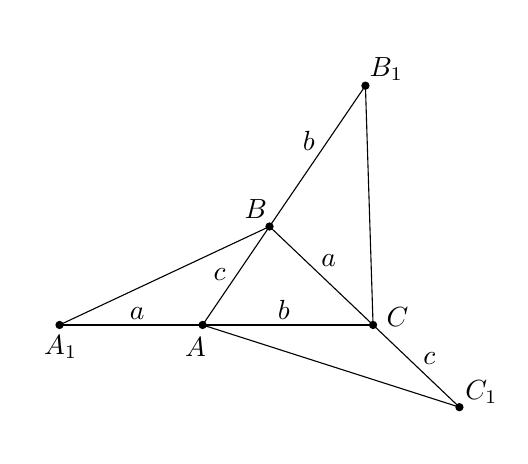
\begin{tikzpicture}[line cap=round,line join=round,>=triangle 45,x=0.40465788199366837cm,y=0.40465788199366837cm]
\clip(-6.81,-3.79) rectangle (8.02,9.03);
\draw (-5.81,-0.3)-- (0.78,2.79);
\draw (3.79,7.21)-- (4.03,-0.3);
\draw (-1.32,-0.3)-- (6.74,-2.88);
\draw (-5.81,-0.3)-- (-1.32,-0.3);
\draw (-1.32,-0.3)-- (0.78,2.79);
\draw (0.78,2.79)-- (3.79,7.21);
\draw (0.78,2.79)-- (4.03,-0.3);
\draw (4.03,-0.3)-- (6.74,-2.88);
\draw (-1.32,-0.3)-- (4.03,-0.3);
\fill [color=black] (-1.32,-0.3) circle (1.5pt);
\draw[color=black] (-1.54,-1.0) node {$A$};
\fill [color=black] (0.78,2.79) circle (1.5pt);
\draw[color=black] (0.35,3.35) node {$B$};
\fill [color=black] (4.03,-0.3) circle (1.5pt);
\draw[color=black] (4.8,-0.06) node {$C$};
\fill [color=black] (-5.81,-0.3) circle (1.5pt);
\draw[color=black] (-5.77,-1.0) node {$A_1$};
\fill [color=black] (3.79,7.21) circle (1.5pt);
\draw[color=black] (4.45,7.74) node {$B_1$};
\fill [color=black] (6.74,-2.88) circle (1.5pt);
\draw[color=black] (7.43,-2.4) node {$C_1$};
\draw[color=black] (-3.37,0.07) node {$a$};
\draw[color=black] (-0.79,1.27) node {$c$};
\draw[color=black] (2.01,5.48) node {$b$};
\draw[color=black] (2.64,1.73) node {$a$};
\draw[color=black] (1.23,0.18) node {$b$};
\draw[color=black] (5.8,-1.35) node {$c$};
\end{tikzpicture}
}
\end{center}
\caption*{A 4. feladathoz.}
\end{figure}
Ismert (könnyen belátható), hogy
\[\frac{T_{AA_1B}}{T_{ABC}}=\frac a b, \quad \frac{T_{BB_1C}}{T_{ABC}}=\frac b c, \quad \frac{T_{CC_1A}}{T_{ABC}}=\frac c a\]
A három egyenletet összeszorozva a következőt kapjuk:
\[\frac{T_{AA_1B}\cdot T_{BB_1C}\cdot T_{CC_1A}}{T_{ABC}^3}=1\textrm{, azaz}\]
\[T_{AA_1B}\cdot T_{BB_1C}\cdot T_{CC_1A}=T_{ABC}^3.\]
Utóbbi összefüggés lehetőséget ad a számtani és mértani közép közti egyenlőtlenség al\-kal\-ma\-zá\-sá\-ra.
\[T_{ABC}=\sqrt[3]{T_{AA_1B}\cdot T_{BB_1C}\cdot T_{CC_1A}}\le\frac{T_{AA_1B}+ T_{BB_1C}+ T_{CC_1A}}{3}\textrm{, azaz}\]
\[3T_{ABC}\le T_{AA_1B}+ T_{BB_1C}+ T_{CC_1A}.\]
Ezzel az állítást bebizonyítottuk.
\medskip


\vonal
{\bf 5. feladat: } 
Legfeljebb hány oldalú az a konvex sokszög, amely feldarabolható olyan de\-rék\-szö\-gű háromszögekre, amelyek hegyesszögei 30 és 60 fokosak? (A feldarabolás során csak ilyen háromszög keletkezhet, másféle sokszög nem).

\ki{Kiss Sándor}{Nyíregyháza}\medskip

{\bf Megoldás: } Tegyük fel, hogy egy konvex sokszög feldarabolható a kívánt módon.

Mivel a felosztásban szereplő háromszögek minden szöge $30^\circ$ egész számú többszöröse, u\-gyan\-ez igaz a sokszög minden egyes szögére, vagyis azok legfeljebb $150^\circ$-os szögek lehetnek.

Ennek megfelelően a sokszög minden külső szöge legalább $30^\circ$-os.

Mivel ezek összege $360^\circ$, a sokszögnek legfeljebb 12 oldala lehet.

\begin{figure}[htpb!]
\begin{center}
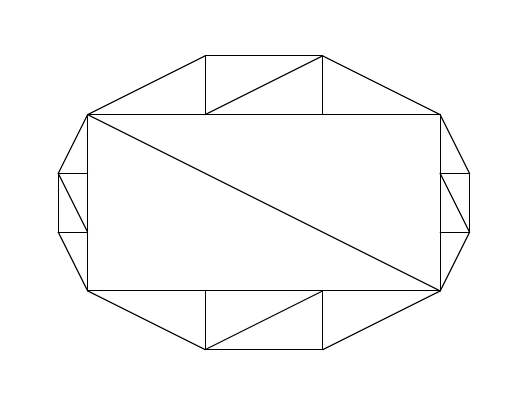
\begin{tikzpicture}[line cap=round,line join=round,>=triangle 45,x=0.7462686567164178cm,y=0.7462686567164178cm]
\clip(-1.02,-1.6) rectangle (7.02,4.48);
\draw (0,3)-- (0,0);
\draw (0,0)-- (6,0);
\draw (6,0)-- (0,3);
\draw (6,3)-- (6,0);
\draw (0,3)-- (6,3);
\draw (2,4)-- (4,4);
\draw (4,4)-- (2,3);
\draw (2,3)-- (2,4);
\draw (2,4)-- (0,3);
\draw (4,4)-- (6,3);
\draw (4,4)-- (4,3);
\draw (2,-1)-- (4,-1);
\draw (4,-1)-- (6,0);
\draw (0,0)-- (2,-1);
\draw (2,-1)-- (2,0);
\draw (4,0)-- (2,-1);
\draw (4,-1)-- (4,0);
\draw (-0.5,2)-- (0,3);
\draw (-0.5,1)-- (0,0);
\draw (-0.5,1)-- (0,1);
\draw (0,2)-- (-0.5,2);
\draw (-0.5,2)-- (0,1);
\draw (-0.5,2)-- (-0.5,1);
\draw (6,0)-- (6.5,1);
\draw (6,2)-- (6.5,1);
\draw (6,3)-- (6.5,2);
\draw (6.5,2)-- (6,2);
\draw (6,1)-- (6.5,1);
\draw (6.5,2)-- (6.5,1);
\end{tikzpicture}
\end{center}
\caption*{Az 5. feladathoz.}
\end{figure}
Az ábrán egy megfelelő 12 oldalú sokszöget láthatunk. Ez úgy keletkezett, hogy először két megfelelő egybevágó háromszöget egy téglalappá illesztettünk össze. Ezután a hosszabbik oldalak fölé harmad ekkora háromszögekből összerakott szimmetrikus trapézokat  illesztettünk, és hasonlóképpen jártunk el a rövidebb oldalakat illetően is.
\medskip


\vonal
{\bf 6. feladat: } 
A 957 háromjegyű szám mögé írjunk három számjegyet úgy, hogy a kapott hatjegyű szám osztható legyen 9-cel, 5-tel és 7-tel is! Melyek ezek a háromjegyű számok?

\ki{Pintér Ferenc}{Nagykanizsa}\medskip

{\bf Megoldás: } Mivel az 5, 7 és 9 páronként relatív prímek, ezért a keresett hatjegyű számnak oszthatónak kell lenni $9\cdot7\cdot5 = 315$-tel.

Másrészt $957000=3038\cdot315 + 30$ , ezért a keresett számok $957\overline{abc}=3038\cdot315 + 30 + \overline{abc}$ alakúak, ahonnan $30 + \overline{abc}$ lehetséges értékei $315$, $2\cdot315 = 630$ vagy $3\cdot315 = 945$ lehetnek, így $\overline{abc}$ vagy 285, vagy 600, vagy 915.

\end{document}